\chapter{Theoretische Grundlagen}\label{ch:theorieGrundlagen}
\section{Elementarladung}\label{sec:elementarladung}
\subsection{Definition}\label{sub:definition}
Die Elementarladung wird physikalisch definiert als,

\begin{equation}\label{eq:definition}
 q  =  n \cdot e \:  \Leftrightarrow \: e = \frac{q}{n} \quad | \ n \in \mathbb{Z}
\end{equation}

\noindent Diese Definition bedeutet nichts anderes, als dass alle möglichen Ladungen ganzzahlige Vielfache der Elementarladung $e$ sind. Diese Erkenntnis bekommt man über den Millikan-Versuch, der aufzeigt, dass sich die Ladungen von Körpern nicht kontinuierlich verteilen, sondern nur in Etagen vorkommen. 

Die Elementarladung besitzt die Einheit Coulomb C. Sie steht als Einheitssymbol für die physikalische Grösse der Ladung $[Q]$. Manchmal wird anstatt Coulomb auch die alternative Schreibweise, die Amperesekunde, verwendet. Das soll Sie aber nicht verwirren, denn die Einheit Coulomb setzt sich aus dem Ampere $[I]$ und der Zeit $[t]$ zusammen. Formal ausgedrückt bedeutet dass: $I \cdot t = Q$. 

\subsection{Eigenschaften}\label{sub:eigenschaften}
Wie oben in \autoref{sec:elementarladung} hergeleitet, hat die Elementarladung die Eigenschaft, dass sie die kleinst mögliche Ladungseinheit in der Natur ist. Kontrovers wird es wenn man Ihnen jetzt sagt das auch drittel Elementarladungen möglich sind. Ein Proton, das die Ladung 1e beträgt, besteht aus drei kleinsten Elementarteilchen, den Quarks. Quarks sind die kleinsten im Moment bekannten Elementarteilchen und sie sind die Bausteine der Materie. Es gibt verschiedene Arten von Quarks, wir beschäftigen uns aber nur mit den Up und Down Quarks. Das Proton besteht aus zwei Up-Quarks und einem Down-Quark. in der folgenden \autoref{tab:quark_tabelle} kann man die verschiedenen Ladungen der Quarks sehen. Wenn man diese Ladungen nun zusammenrechnet kommt man wieder auf die Elementarladung e. 

\begin{equation}\label{eq:mathematische_zusammensetzung_von_qurks}
	2 \cdot \left(\frac{2}{3}e\right)  + 1 \cdot \left( -\frac{1}{3}e\right) 
	= \frac{4}{3}e - \frac{1}{3}e = 1e
\end{equation}

\noindent Wie in \autoref{eq:mathematische_zusammensetzung_von_qurks} gezeigt, kann die Elementarladung auch aus Bruchteilen von sich selber bestehen. Wieso hat man jetzt genau die Ladung eines Elektron oder Proton als Elementarladung festgelegt? Das ist sehr einfach zu beantworten, wenn man die Verhaltensweise von Quarks kennt. Quarks kommen nie einzeln in der Natur von, sondern nur in sogenannten Quark-Gluon-Plasmen. Einfach ausgedrückt nur als Pärchen in einem Proton oder Neutron.

%\begin{figure}[h]\label{fig:quarkTabelle}
	%\begin{center}
		%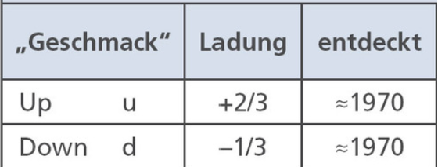
\includegraphics[scale=1]{bilder/pdf/quark_tabelle.pdf}
	%	\caption{Tabelle Ladung von Quarks}
%	\end{center}
%\end{figure}

\begin{table}[ht]
	\begin{center}
		\begin{tabular}{l|l}
			\multicolumn{2}{c}{\textit{\textbf{Quark Tabelle}}} \\
			\hline
			Art & Ladung \\
			\hline
			Up u & $+ \frac{2}{3}e$ \\
			\hline
			Down d & $- \frac{1}{3}e$\\
			\hline
		\end{tabular}
	\end{center}
	\caption{Up-Down-Quark Ladungen}
	\label{tab:quark_tabelle}
\end{table}

\section[Historische Methoden]{Historische Methoden zur Bestimmung der Elementarladung}
\subsection{Thomsonsche Methode}\label{sub:thomson}
In dieser Arbeit geht es hauptsächlich um den Millikan-Versuch, zur Bestimmung der Elementarladung. Andere Methoden sind aber dennoch nennenswert. Zum Beispiel das Thomsonsche Experiment. Dabei geht es um einen Versuch, der ein Elektronenstrahl durch ein magnetisches Feld schiesst. Dabei wird der Strahl durch die Lorenzkraft abgelenkt und Joseph John {\scshape Thomson} konnte, durch verändern des Magnetfeldes, das Verhältnis von Masse und Ladung $\frac{e}{m}$ entdecken. Durch dieses Verhältnis konnte er die Elementarladung noch nicht bestimmen. Erst später als man die Masse eines Elektron entdeckte, konnte man indirekt über dieses Verhältnis auf die Ladung zurückschliessen. 

\subsection{Elektrolyse}\label{sub:elektrolyse}
Eine andere Methode, die Elementarladung zu ermitteln, funktioniert mithilfe der Elektrolyse. Bei der Elektrolyse wird eine Spannung angelegt um chemische Reaktionen (zum Beispiel Zersetzung von Molekülen) in einer ionischen Lösung zu erzwingen. Dabei kann man durch Messungen der Spannung und Anzahl Ionen, die gewandert sind, auf die Elementarladung schliessen. 

Mit beiden dieser Methoden kann man die Elementarladung indirekt bestimmen. Sie sind für diese Arbeit sicher nennenswert, jedoch kann man mithilfe des Millikan Versuchs viel direkter Ladungen kleinster Partikel messen.

\section{Theorie des Versuchs}\label{sec:versuchsTheorie}
Da wir die anderen Methoden nur kurz angeschnitten haben, wird der Millikan Versuch jetzt genauer erklärt oder zumindest die Theorie dahinter. 

Wir beginnen mit einem Öltröpfchen im Freien Fall. Folgende \autoref{fig:freierFall} ist dazu zu sehen.

\begin{figure}[h]
	\begin{center}
		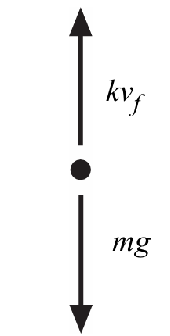
\includegraphics[scale=0.5]{bilder/pdf/Abbildung1_FreierFall.pdf}
		\caption{Öltröpfchen im Freien Fall}
		\label{fig:freierFall}
	\end{center}
\end{figure}

\noindent In \autoref{fig:freierFall} sehen wir welche Kräfte auf ein Öltröpfchen im freien Fall wirken. Nach unten haben wir die Gewichtskraft, die Abhängig ist von der Masse \textbf{$m$} und dem Ortsfaktor \textbf{$g$}. Das Öltröpfchen fällt in der Luft und hat seine Endgeschwindigkeit erreicht (die dazu benötigte Zeit beträgt wenige Millisekunden). Die Kraft, die nach oben zeigt, ist die Reibungskraft der Luft. Sie ist abhängig von der Fall- bzw. Endgeschwindigkeit \textbf{$v_f$} und dem Reibungskoeffizienten \textbf{$k$} von Luft und dem Tröpfchen.
Diese Kräfte sind genau gleich gross, weil sie in einem Kräftegleichgewicht sind. 

\begin{equation}\label{eq:kräfteFreierFall}
	mg \ = \ kv_f
\end{equation}   

\noindent Nun setzen wir dieses Öltröpfchen in ein elektrisches Feld. Mit den Kräftevektoren eingezeichnet, sieht das so aus.

\begin{figure}[h]
	\begin{center}
		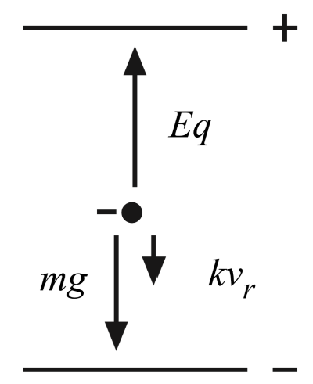
\includegraphics[scale=0.5]{bilder/pdf/Abbildung2_elektrischesFeld.pdf}
		\caption{Öltröpfchen im elektrischen Feld}
		\label{fig:elektrischesFeld}
	\end{center}
\end{figure}

\noindent Die elektrische Kraft, die in \autoref{fig:elektrischesFeld} nach oben zeigt, ist abhängig von der elektrischen Feldstärke $E$ und der Ladung $q$ des Tröpfchen. Da die elektrische Kraft nun grösser als die Gewichtskraft ist, steigt das Tröpfchen. Wie wir schon oben im Freien Fall behandelt haben, gibt es wieder eine Reibungskraft der Luft die entgegengesetzt der Bewegungsrichtung verläuft. Dieses Mal ist sie aber nicht von der Fallgeschwindigkeit abhängig, sondern von der Steiggeschwindigkeit $v_r$ (steig auf Englisch: rise) und wie oben von dem Reibungskoeffizienten der Luft $k$. Wenn man jetzt diese Vektoren algebraisch addiert, kommt man auf folgende Gleichung.

\begin{equation}\label{eq:elektrischesFeld}
	Eq \ = \ mg \cdot kv_r
\end{equation}

\noindent Nun kann man nach $q$ umstellen und den Reibungskoeffizienten $k$ mithilfe der \autoref{eq:kräfteFreierFall} eliminieren. 

\begin{equation}\label{eq:hauptgleichung}
	q \ = \ \frac{mg \cdot (v_f + v_r)}{Ev_f}
\end{equation}

\noindent Die Masse eines Öltröpfchens zu bestimmen, ist in diesem Fall fast unmöglich. Aus diesem Grund versucht man über die Dichte des Öls $\rho$, und das Volumen der Ölkugel, auf die Masse zu kommen. Der Zusammenhang von Dichte und Masse sieht folgendermassen aus: $\rho \ = \ \frac{m}{V} \ \Leftrightarrow \ m \ = \ \rho \cdot V$. Das Volumen kann jetzt noch ausgerechnet werden mithilfe des Radius $a$. Setzt man nun alles zusammen, kommt man auf folgende Formel für die Masse eines Öltröpfchens. 

\begin{equation}\label{eq:masseFormel}
	mg \ = \ \frac{4}{3} \pi a^3 \rho g
\end{equation}

\noindent Wir können jetzt dieses $m$ mit dem $m$ in \autoref{eq:hauptgleichung} substituieren.

\begin{equation}\label{eq:ladungFormel}
	q \ = \ \frac{4\pi a^3\rho g (v_f + v_r)}{3(Ev_f)}
\end{equation}

\noindent Das neue Problem wird jetzt der Radius $a$ sein. Die Tröpchen sind zu klein, um den Radius zu messen. Die Lösung des Problems finden wir im stokesschen Reibungsgesetz $(F_f \ = \ 6\pi \eta a v_f)$. Es zeigt den Zusammenhang von Fallgeschwindigkeit und Reibungskraft der Luft. Diese Formel beschreibt, wie sich ein Kugelförmiges Objekt in einem viskosem Medium verhält. Dieses Gesetz hängt von der Reibungszahl der Luft $\eta$ und der Fallgeschwindigkeit $v_f$ ab. Wir können diesen Ausdruck mit dem rechten Ausdruck von Gleichung \ref{eq:masseFormel} gleichsetzen. Wenn man nach $a$ auflöst erhält man:

\begin{equation}\label{eq:stokesRadius}
	a \ = \ \sqrt{\frac{9\eta v_f}{2\rho g}}
\end{equation}

\noindent Das stokessche Reibungsgesetz wird leider inkorrekt wenn die Fallgeschwindigkeit weniger als 0.1 cm/s beträgt. Da wir es im Experiment mit Fallgeschwindigkeiten zwischen 0.01 und 0.001 cm/s (zwischen $10^-4$ und $10^-6$ m/s) zu tun haben, müssen wir das Reibungsgesetz mit einem Korrekturfaktor multiplizieren. Die effektive Viskosität resultiert aus:

\begin{equation}\label{eq:effViskosität}
	\eta_{eff} \ = \ \eta \left( \frac{1}{1 + \frac{b}{pa}} \right) 
\end{equation}

\noindent $b$ ist dabei eine Konstante und $p$ ist der atmosphärische Druck in Pascal. 

\noindent Nun wird $\eta_{eff}$ in Gleichung \ref{eq:effViskosität} für $\eta$ in Gleichung \ref{eq:stokesRadius} substituiert. 

\begin{equation}\label{eq:korrekturRadius}
	a \ = \ \sqrt{\frac{9\eta v_f}{2\rho g} \left( \frac{1}{1 + \frac{b}{pa}}\right)}
\end{equation}

\noindent \autoref{eq:effViskosität} enthält den Radius $a$. Das Problem ist, dass wir einen Term für $a$ gefunden haben, der $a$ aber enthält. Der Ausdruck für $a$ in \autoref{eq:korrekturRadius} kann in eine quadratische Gleichung umgewandelt werden:

\begin{equation}\label{eq:quadraticRadius}
	\begin{split}
		a & \ = \ \sqrt{\frac{9\eta v_f}{2\rho g} \left( \frac{1}{1 + \frac{b}{pa}}\right)} \\
		a^2 & \ = \ \frac{9\eta v_f}{2\rho g} \left( \frac{1}{1 + \frac{b}{pa}}\right) \\
		a^2 + \frac{b}{p}a & \ = \ \frac{9\eta v_f}{2\rho g} \\
		a^2 + \frac{b}{p}a - \frac{9\eta v_f}{2\rho g} & \ = \ 0
	\end{split}
\end{equation} 

\noindent Jetzt wird \autoref{eq:quadraticRadius} nach $a$ aufgelöst:

\begin{equation}\label{eq:qRadius}
	a \ = \ \sqrt{\left( \frac{b}{2p}\right)^2 + \frac{9\eta v_f}{2\rho g}} - \frac{b}{2p}
\end{equation}

\noindent Es ist zu beachten, dass, nicht wie bei \autoref{eq:korrekturRadius}, jetzt kein $a$ im Ausdruck mehr vorkommt. Jetzt wird der komplette Term für $a$ in Gleichung \ref{eq:ladungFormel} ersetzt.

\begin{equation}\label{eq:ladungMitEingesetzR}
	q \ = \ \frac{4\pi \left[ \sqrt{\left( \frac{b}{2p}\right)^2 + \frac{9\eta v_f}{2\rho g}} - \frac{b}{2p} \right]^3 \rho g(v_f + v_r) }{3(Ev_f)}
\end{equation}

\noindent Die Elektrische Feldstärke $E$ kann auch so ausgedrückt werden:

\begin{equation}\label{eq:elektrischeFeldstärke}
	E \ = \ \frac{V}{d}
\end{equation}

\noindent Wenn jetzt $E$ aus Gleichung \ref{eq:ladungMitEingesetzR} mit $E$ aus \autoref{eq:elektrischeFeldstärke} ersetzt wird und die ganze Gleichung noch schöner umgeformt wird, resultiert daraus:

\begin{equation}\label{eq:letzteFormel}
	q \ = \ \frac{4\pi}{3} \cdot \left[ \sqrt{\left( \frac{b}{2p}\right)^2 + \frac{9\eta v_f}{2\rho g}} - \frac{b}{2p} \right]^3 \cdot \frac{\rho gd(v_f + v_r)}{Vv_f}
\end{equation}

\noindent Die Quelle für all diese Berechnungen basieren auf \parencite{instructionManual}




	

